
\documentclass[tikz,border=5pt]{standalone}
\usepackage{amsmath,amssymb}
\usetikzlibrary{arrows.meta,positioning,calc,shapes.geometric}

\begin{document}
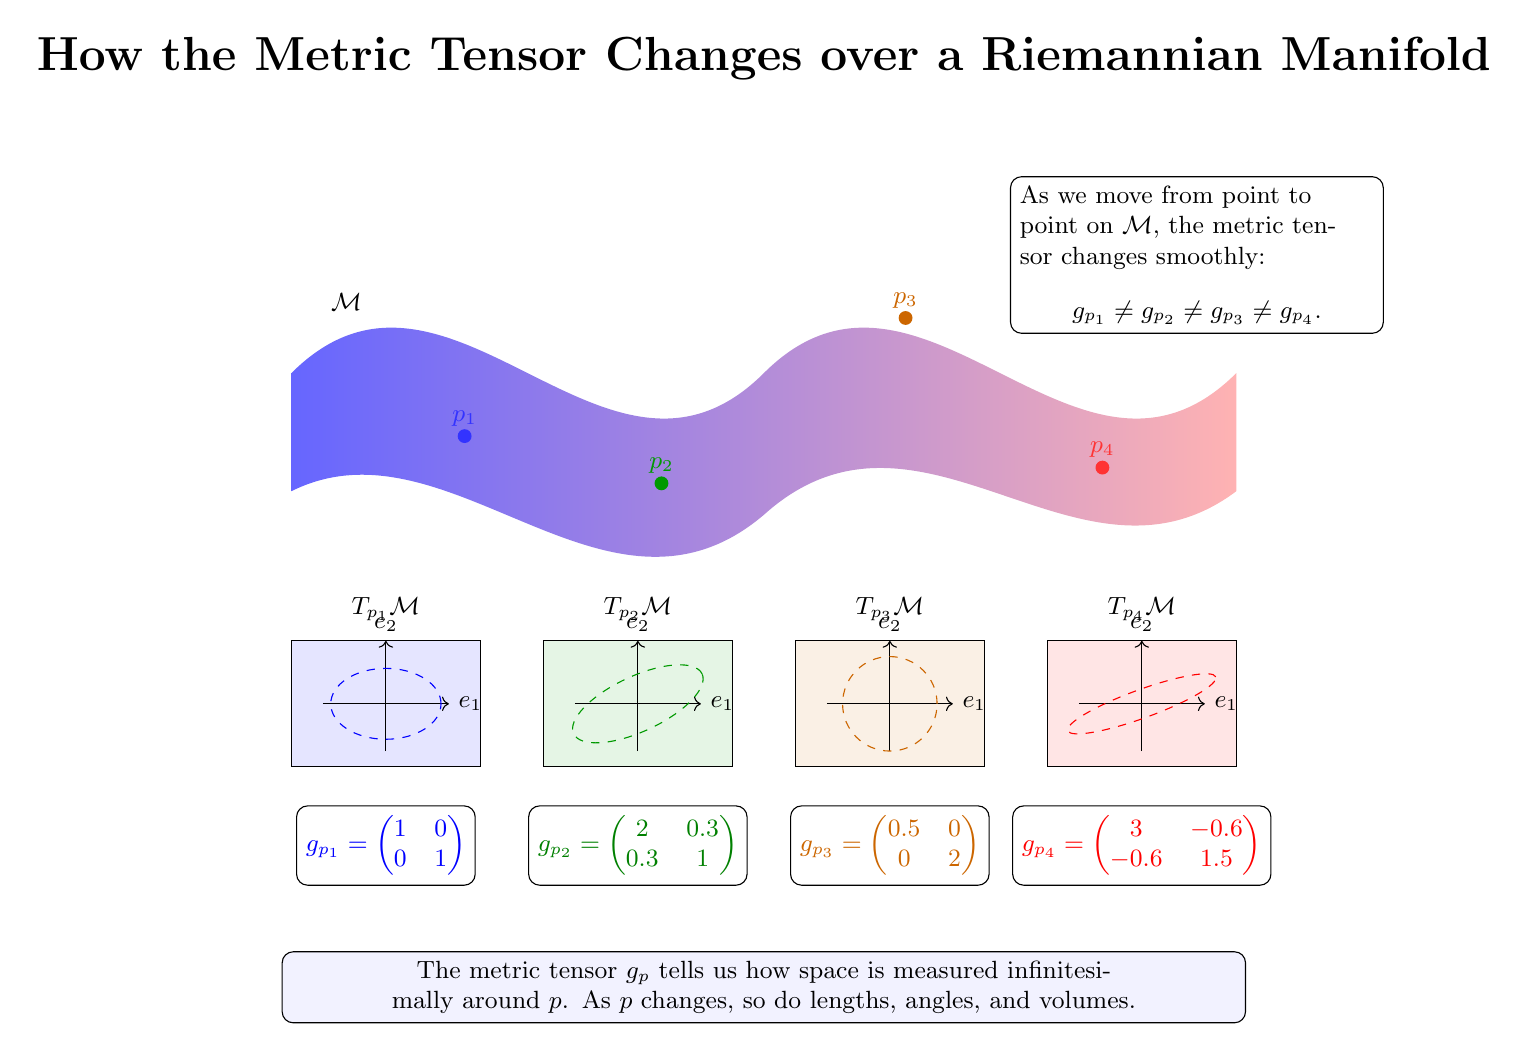
\begin{tikzpicture}[font=\small]

% Title
\node[font=\bfseries\LARGE] at (0,8) {How the Metric Tensor Changes over a Riemannian Manifold};

% Manifold (stylized)
\shade[left color=blue!60,right color=red!30]
(-6,4) .. controls (-4,6) and (-2,2) .. (0,4)
.. controls (2,6) and (4,2) .. (6,4)
-- (6,2.5)
.. controls (4,1) and (2,4) .. (0,2.2)
.. controls (-2,0.5) and (-4,3.5) .. (-6,2.5) -- cycle;

\node at (-5.3,4.9) {$\mathcal M$};

% Points
\fill[blue!80] (-3.8,3.2) circle (2.5pt) node[above] {$p_1$};
\fill[green!60!black] (-1.3,2.6) circle (2.5pt) node[above] {$p_2$};
\fill[orange!80!black] (1.8,4.7) circle (2.5pt) node[above] {$p_3$};
\fill[red!80] (4.3,2.8) circle (2.5pt) node[above] {$p_4$};

% Explanatory box
\node[draw,rounded corners,align=left,text width=4.5cm] at (5.5,5.5)
{As we move from point to point on $\mathcal M$, the metric tensor changes smoothly:
\[g_{p_1}\neq g_{p_2}\neq g_{p_3}\neq g_{p_4}.\]};

% Tangent spaces
\foreach \x/\c/\lab in {-4.8/blue/$T_{p_1}\mathcal M$,
                         -1.6/green!60!black/$T_{p_2}\mathcal M$,
                         1.6/orange!80!black/$T_{p_3}\mathcal M$,
                         4.8/red/$T_{p_4}\mathcal M$}
{
  \begin{scope}[shift={(\x,-0.2)}]
    \draw[fill=\c!10] (-1.2,-0.8) rectangle (1.2,0.8);
    \draw[->] (-0.8,0)--(0.8,0) node[right] {$e_1$};
    \draw[->] (0,-0.6)--(0,0.8) node[above] {$e_2$};
    \node at (0,1.2) {\lab};
  \end{scope}
}

% Unit balls
\draw[blue,dashed] (-4.8,-0.2) ellipse (0.7 and 0.45);
\draw[green!60!black,dashed,rotate around={25:(-1.6,-0.2)}] (-1.6,-0.2) ellipse (0.9 and 0.35);
\draw[orange!80!black,dashed] (1.6,-0.2) ellipse (0.6 and 0.6);
\draw[red,dashed,rotate around={20:(4.8,-0.2)}] (4.8,-0.2) ellipse (1.0 and 0.18);

% Metric matrices
\node[draw,rounded corners,text=blue] at (-4.8,-2)
{$g_{p_1}=\begin{pmatrix}1&0\\0&1\end{pmatrix}$};

\node[draw,rounded corners,text=green!50!black] at (-1.6,-2)
{$g_{p_2}=\begin{pmatrix}2&0.3\\0.3&1\end{pmatrix}$};

\node[draw,rounded corners,text=orange!80!black] at (1.6,-2)
{$g_{p_3}=\begin{pmatrix}0.5&0\\0&2\end{pmatrix}$};

\node[draw,rounded corners,text=red] at (4.8,-2)
{$g_{p_4}=\begin{pmatrix}3&-0.6\\-0.6&1.5\end{pmatrix}$};

% Bottom note
\node[draw,rounded corners,fill=blue!5,text width=12cm,align=center]
at (0,-3.8)
{The metric tensor $g_p$ tells us how space is measured infinitesimally around $p$.
As $p$ changes, so do lengths, angles, and volumes.};

\end{tikzpicture}
\end{document}
